\let\negmedspace\undefined
\let\negthickspace\undefined
\documentclass[journal]{IEEEtran}
\usepackage[a5paper, margin=10mm, onecolumn]{geometry}
%\usepackage{lmodern} % Ensure lmodern is loaded for pdflatex
\usepackage{tfrupee} % Include tfrupee package

\setlength{\headheight}{1cm} % Set the height of the header box
\setlength{\headsep}{0mm}     % Set the distance between the header box and the top of the text

\usepackage{gvv-book}
\usepackage{gvv}
\usepackage{cite}
\usepackage{amsmath,amssymb,amsfonts,amsthm}
\usepackage{algorithmic}
\usepackage{graphicx}
\usepackage{textcomp}
\usepackage{xcolor}
\usepackage{txfonts}
\usepackage{listings}
\usepackage{enumitem}
\usepackage{mathtools}
\usepackage{gensymb}
\usepackage{comment}
\usepackage[breaklinks=true]{hyperref}
\usepackage{tkz-euclide} 
\usepackage{listings}
% \usepackage{gvv}                                        
\def\inputGnumericTable{}                                 
\usepackage[latin1]{inputenc}                                
\usepackage{color}                                            
\usepackage{array}                                            
\usepackage{longtable}                                       
\usepackage{calc}                                             
\usepackage{multirow}                                         
\usepackage{hhline}                                           
\usepackage{ifthen}                                           
\usepackage{lscape}
\usepackage{circuitikz}
\tikzstyle{block} = [rectangle, draw, fill=blue!20, 
    text width=4em, text centered, rounded corners, minimum height=3em]
\tikzstyle{sum} = [draw, fill=blue!10, circle, minimum size=1cm, node distance=1.5cm]
\tikzstyle{input} = [coordinate]
\tikzstyle{output} = [coordinate]

\begin{document}


\bibliographystyle{IEEEtran}
\vspace{3cm}

\title{4.3.41}
\author{EE25BTECH11051 - Shreyas Goud Burra}
\maketitle
{\let\newpage\relax\maketitle}

\renewcommand{\thefigure}{\theenumi}
\renewcommand{\thetable}{\theenumi}
\setlength{\intextsep}{10pt}


\numberwithin{equation}{enumi}
\numberwithin{figure}{enumi}
\renewcommand{\thetable}{\theenumi}

\textbf{Question}\\
The cartesian equation of a line is $\frac{x-5}{3}=\frac{y+4}{7}=\frac{z-6}{2}$. Write its vector form.\\

\solution

Given cartesian equation of line is

\begin{align}
    \frac{x-5}{3}=\frac{y+4}{7}=\frac{z-6}{2}=\lambda
    \label{0.1}
\end{align}

We know the vector form of a line is given by,
\begin{align}
    \textbf{x} = \textbf{h}+k\textbf{m}
    \label{0.2}
\end{align}

Where \textbf{x} is a point on the given line, \textbf{h} is a known point on that line, \textbf{m} is the slope of the line and k is an arbitrary real constant.\\

From \ref{0.1}, we can determine a point on the line taking $\lambda =0$
\begin{align}
    \frac{x-5}{3}=\frac{y+4}{7}=\frac{z-6}{2}=0 \implies x=5, y=-4, z=6
    \label{0.3}
\end{align}

\begin{align}
    \implies \textbf{h} = \myvec{5\\-4\\6}
    \label{0.4}
\end{align}

We can get the ratio of direction cosines from \ref{0.1}
\begin{align}
    \text{ratio}=3:7:2 \implies \textbf{m} = \myvec{3\\7\\2}
    \label{0.5}
\end{align}

Substituting \ref{0.4} and \ref{0.5} in \ref{0.2}, we get

\begin{align}
    \textbf{x} = \myvec{3\\-4\\6} + k\myvec{3\\7\\2}
    \label{0.6}
\end{align}

The plot for the given question is given below,

\begin{figure}[H]
    \centering
    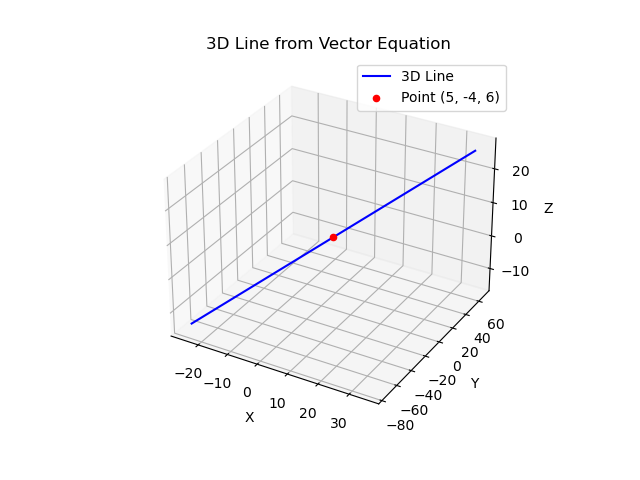
\includegraphics[width=0.8\columnwidth]{figs/fig1.png}
    \caption{3D Plot}
    \label{3D Plot}
\end{figure}

\end{document}
